\chapter{\textbf{Technical Specifications of Hardware and Software}}
This chapter is about the specification of different module which was used for this project viz their current rating,voltage rating and remarks of these components.This chapter is meant to explain how the components work in the project.

\section{Hardware requirements}
\begin{enumerate}
\item	NodeMCU
\item	LPG Gas sensor Module MQ-6
\item	DHT-11 Sensor
\item	Solenoid Valve (12V)
\item   DC Pump (12V)
\item	300 MBPS Router
\item	Jumper Wires
\item	Relay Modules and etc.
\end{enumerate}
\section{Specifications of components}
\subsection{NodeMCU Specifications}
NodeMCU is an open source IoT platform. It includes firmware which runs on the ESP8266 Wi-Fi SoC from Espressif Systems, and hardware which is based on the ESP-12 module. The term "NodeMCU" by default refers to the firmware rather than the development kits. The firmware uses the Lua scripting language. It is based on the eLua project, and built on the Express if Non-OS SDK for ESP8266. It uses many open source projects, such as lua-cjson and spiffs [36]. Technical specifications are given below:

\begin{enumerate}
  \item Voltage:3.3V.
\item	Wi-Fi Direct (P2P), soft-AP.
\item	Current consumption: 10uA~170mA.
\item	Flash memory attachable: 16MB max (512K normal).
\item	Integrated TCP/IP protocol stack.
\item	Processor: Tensilica L106 32-bit.
\item	Processor speed: 80~160MHz.
\item	RAM: 32K + 80K.
\item	GPIOs: 17 (multiplexed with other functions).
\item	Analog to Digital: 1 input with 1024 step resolution.
\item	+19.5dBm output power in 802.11b mode
\item	802.11 support: b/g/n.
\end{enumerate}

A graphical schematic of NodeMCU is given below in Figure \ref{fig1} [36].

\begin{figure}[h]
  \centering
  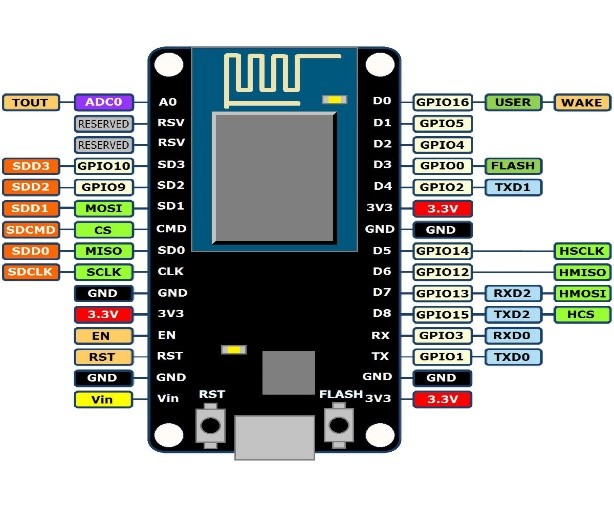
\includegraphics[width=3in]{1}
  \caption{NodeMCU}\label{fig1}
\end{figure}

While writing GPIO code on NodeMCU, you can’t address them with actual GPIO Pin Numbers. There are different I/O Index numbers assigned to each GPIO Pin which is used for GPIO Pin addressing. Figure-2.2 shows a graphical representation of NodeMCU pin settings. Refer following Table \ref{tab1} to check I/O Index of NodeMCU GPIO Pins –

\begin{table}
  \caption{NodeMCU pin settings}\label{tab1}
  \centering
  \begin{tabular}{|p{1in}|p{1.5in}|}
    \hline
    \textbf{GPIO Pin} & I\textbf{/O Index Number}\\[2ex] \hline
    GPIO0 &  3\\[2ex] \hline
    GPIO1 &  10\\[2ex] \hline
    GPIO2 &  4\\[2ex] \hline
    GPIO3 &  9\\[2ex] \hline
    GPIO4 &  2\\[2ex] \hline
    GPIO5 &  1\\[2ex] \hline
    GPIO6 &  N/A\\[2ex] \hline
    GPIO7 &  N/A\\[2ex] \hline
    GPIO8 &  N/A\\[2ex] \hline
    GPIO9 &  11\\[2ex] \hline
    GPIO10 &  12\\[2ex] \hline
    GPIO11 &  N/A\\[2ex] \hline
    GPIO12 &  6\\[2ex] \hline
    GPIO13 &  7\\[2ex] \hline
    GPIO14 &  5\\[2ex] \hline
    GPIO15 &  8\\[2ex] \hline
    GPIO16 &  0\\[2ex] \hline
  \end{tabular}
\end{table}
\newpage

\begin{figure}[t]
  \centering
  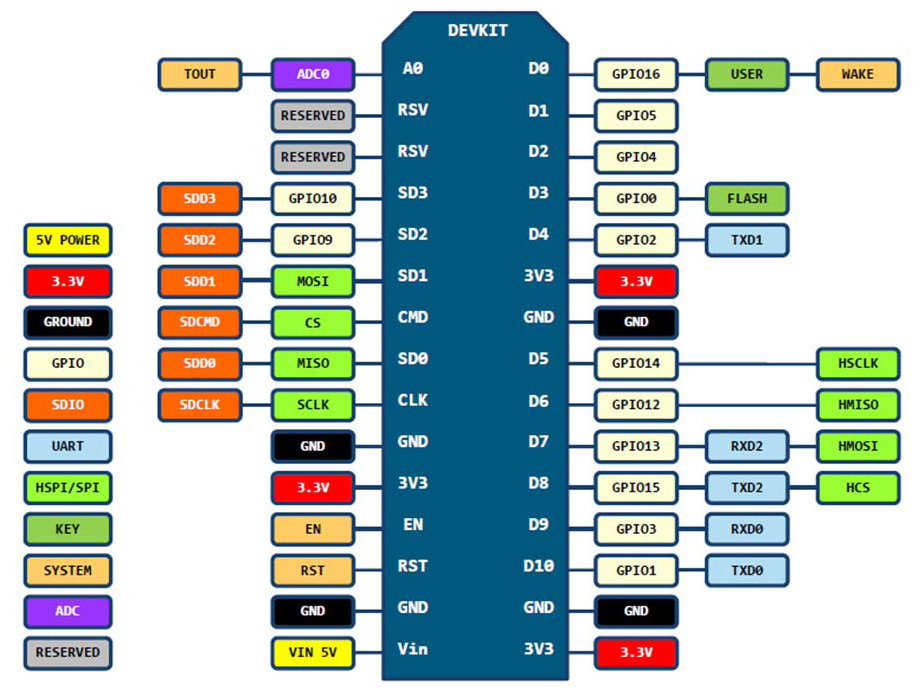
\includegraphics[width=6in]{2}
  \caption{NodeMCU v.1.0 Pin Definition}\label{fig2}
\vspace{.3in}
\end{figure}


The NodeMCU can be programmed with the Arduino software (Arduino IDE). Select "ESP 8266 NodeMCU v.1.0" from the Tools > Board menu. The microcontroller provides pre-burned with a boot loader that allows you to upload new code to it without the use of an external hardware programmer. It communicates using the original STK500 protocol (reference, C header files). It also can bypass the boot loader and program the microcontroller through the ICSP (In-Circuit Serial Programming) header. The NodeMCU has a resettable poly fuse that protects your computer's USB ports from shorts and over current. Although most computers provide their own internal protection, the fuse provides an extra layer of protection. If more than 500mA is applied to the USB port, the fuse will automatically break the connection until the short or overload is removed.\\
\vspace{.3in}
\subsection{Gas sensor MQ-6 Module Specifications}
MQ-6 is a semiconductor type gas sensor which detects the gas leakage. The sensitive material of MQ-6 is tin dioxide (SnO2). It has very low conductivity in clean air. MQ-6 gas sensor has high sensitivity to LPG, concentration level of it is from 200 – 1000 ppm and it also detects the following flammable gases: 1. Propane 2. Hydrogen 3. Methane 4. Butane. Figure \ref{fig3} shows a schematic of MQ-6 gas sensor module [37].\\

\begin{figure}[h]
  \centering
  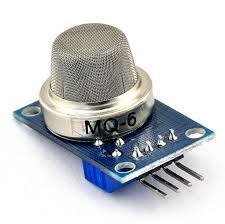
\includegraphics[width=3.6in]{3}
  \caption{MQ-6 Gas sensor}\label{fig3}
\end{figure}

The features of MQ-6 gas sensor are given below:

\begin{enumerate}
  \item Wide detecting scope
\item High sensitivity to combustible gas in wide range
\item Fast response
\item Stable and long life
\item Simple drive circuit
\item Low cost and compact size.
\end{enumerate}

The gas sensor senses the analog value according to the concentration of the gas level in the environment. The concentration range of MQ-6 gas sensor is 200-1000ppm for LPG and use value of Load resistance $(R_L)$ about $20 k\Omega (10 k\Omega to 47 k\Omega)$. When accurately measuring, the proper alarm point for the gas detector should be determined after considering the temperature and humidity influence. The voltage that the sensor outputs changes accordingly to the smoke/gas level that exists in the atmosphere. The sensor outputs a voltage that is proportional to the concentration of smoke/gas. The resistance of the sensor is different depending on the type of the gas. Figure \ref{fig4} shows a schematic of inside circuitry of MQ-6 gas sensor.

\begin{figure}[h]
  \centering
  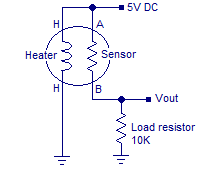
\includegraphics[width=3.5in]{4}
  \caption{MQ-6 circuit.}\label{fig4}
\end{figure}

MQ-6 sensor senses the flammable gases by the increase in temperature when they are oxidized by the heating element. Consider the figure given above. If there is any flammable gas present in the sample, the oxidization of the same gas results in increased temperature and the resistance of the sensor resistor will drop. That means more current will flow through the load resistor and so the voltage across it will shoot up. MQ-6 gas sensor pin description: 1. $D_0$ (Digital Pin), 2. A0 (Analog Pin), 3. VCC (+5V), 4. GND [Graphical illustration in Figure \ref{fig5}].

\begin{figure}[h]
  \centering
  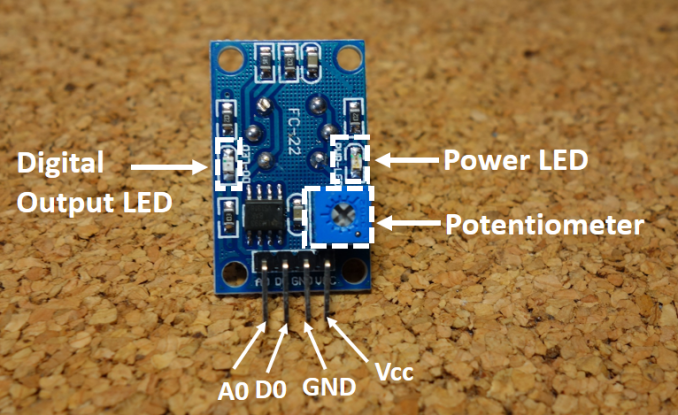
\includegraphics[width=5in]{5}
  \caption{MQ-6 pinout.}\label{fig5}
\end{figure}

The working condition is very important for the sensory performance. Table \ref{tab2} shows the standard working conditions and optimal operations of MQ-6 gas sensor. Sensitivity is also an important factor for the sensory signal calibration. Figure \ref{fig6} and Figure \ref{fig7} shows the sensitive relations of MQ-6 with respect to ppm (Parts per Millions) and Relative Humidity respectively.
\begin{table}[h]
  \caption{Standard Working Condition:}\label{tab2}
  \centering
  \begin{tabular}{|p{.5in}|p{1.5in}|p{1.5in}|p{1.5in}|}
    \hline
    Symbol & Parameter Name & Technical Condition & Remarks\\[1ex] \hline
     $V_C$ & Circuit voltage & $5V\pm0.1$ & AC or DC\\[1ex] \hline
     $V_H$ & Heating voltage & $5V\pm0.1$ & AC or DC\\[1ex] \hline
     $R_L$ & Load resistance & Adjustable & \\[1ex] \hline
     $R_H$ & Heater resistance & $33k.Ohm\pm5\%$ & Room Temperature\\[1ex] \hline
     $P_H$ & Heating consumption & Less than 800mW & \\[1ex]
    \hline
  \end{tabular}
\end{table}
Structure and configuration of MQ-6 gas sensor is shown as Figure\ref{fig6}, sensor composed by micro AL\_2O\_3 ceramic tube, Tin Dioxide (SnO2) sensitive layer, measuring electrode and heater are fixed into a crust made by plastic and stainless steel net. The heater provides necessary work conditions for work of sensitive components. The enveloped MQ-6 have 6 pin ,4 of them are used to fetch signals, and other 2 are used for providing heating current.
\begin{figure}[h]
  \centering
  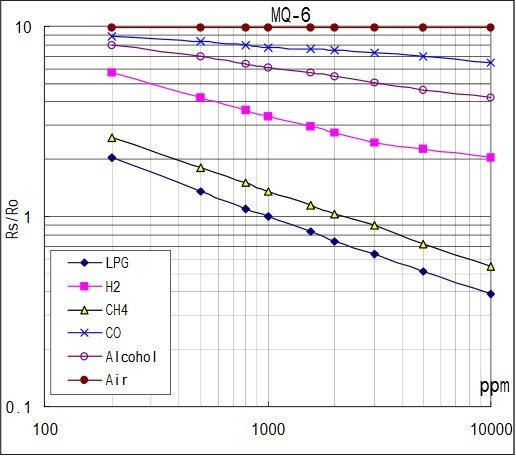
\includegraphics[width=4in]{6}
  \caption{MQ-6 gas sensor sensitivity at optimum conditions [38].}\label{fig6}
\end{figure}
Resistance value of MQ-6 is difference to various kinds and various concentration gases. So, When using this components, sensitivity adjustment is very necessary.Recommend that here calibrated value that detects for 1000 ppm of LPG concentration in air and use value of Load resistance$(R_L)$ about $20 k\Omega (10 k\Omega to 47 k\Omega)$. When accurately measuring, the proper alarm point for the gas detector should be determined after considering the temperature and humidity influence.

\begin{figure}[h]
  \centering
  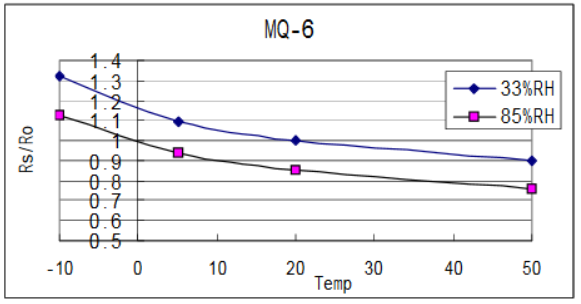
\includegraphics[width=4in]{7}
  \vspace{-.1in}
  \caption{MQ-6 sensor sensitivity with respect to Temperature [38].}\label{fig7}
\end{figure}
Resistance value of MQ-6 is difference to various kinds and various concentration gases. So, when using these components, sensitivity adjustment is very necessary. Recommended that here calibrated value that detects for 1000ppm liquefied petroleum gas (LPG), or 1000ppm iso-butane concentration in air and use value of load resistance that about 20 Kilo-Ohms. When accurately measuring the proper alarm point for the gas detector should be determined after considering the temperature and humidity influence. Applications of MQ-6 gas sensor is given below:
\begin{enumerate}
  \item	Domestic gas leakage detector.
  \item	Industrial combustible gas leakage detector.
  \item	Portable gas leakage detector.
  \item	Concentration level for LPG is 400-1000ppm.
  \item	Circuit voltage is 5V.

\end{enumerate}
\subsection{DHT 11 Humidity \& Temperature Sensor Module Specification}
DHT11 Temperature \& Humidity Sensor features a temperature \& humidity sensor complex with a calibrated digital signal output. By using the exclusive digital-signal-acquisition technique and temperature \& humidity sensing technology, it ensures high reliability and excellent long-term stability. This sensor includes a resistive-type humidity measurement component and an NTC temperature measurement component, and connects to a highperformance 8-bit microcontroller, offering excellent quality, fast response, anti-interference ability and cost-effectiveness.
\begin{figure}[h]
  \centering
  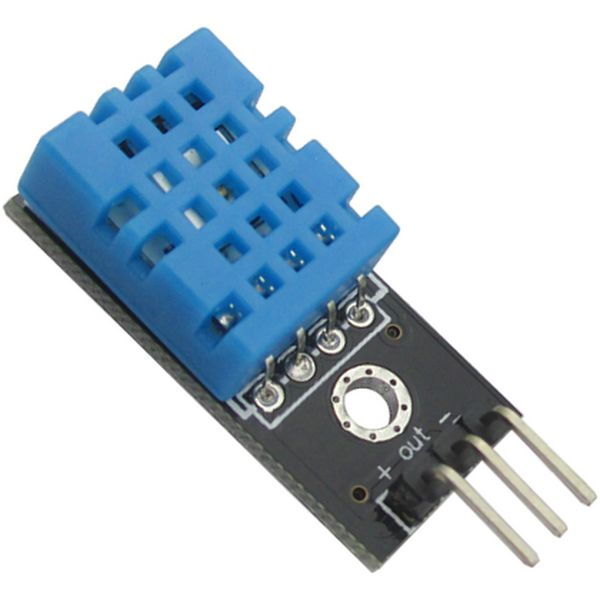
\includegraphics[width=4in]{43}
  \caption{DHT11 Temperature and Humidity sensor Breakout}\label{fig43}
\end{figure}
Each DHT11 element is strictly calibrated in the laboratory that is extremely accurate on humidity calibration. The calibration coefficients are stored as programmes in the OTP memory, which are used by the sensor’s internal signal detecting process\cite{jokar2016intrusion}. The single-wire serial interface makes system integration quick and easy. Its small size, low power consumption and up-to-20 meter signal transmission making it the best choice for various applications, including those most demanding ones. The component is 4-pin single row pin package. It is convenient to
connect and special packages can be provided according to the users.
\newpage
\subsection{DHT11 Temperature \& Humidity Sensor Specification}
\begin{enumerate}
  \item Low cost
\item 3 to 5V power and I/O
\item 2.5mA max current use during conversion (while requesting data)
\item Good for 20-80 \% humidity readings with 5 \% accuracy
\item Good for 0-50 $\circ$ degree C temperature readings $\pm$ 2 $\circ$ degree C accuracy
\item Not more than 1 Hz sampling rate (once every second)
\item Body size 15.5mm x 12mm x 5.5mm
\item 4 pins with 0.1 inch spacing
\end{enumerate}
\subsection{Solenoid Valve Specifications}
\begin{enumerate}
  \item APL-3/2’’-12VDC
  \item	Position: Normally Closed
  \item	Port Size: 1/2" Male NPT
  \item	Voltage: 12V DC
  \item	Body Material: POM Plastic
  \item	Components: Stainless Steel
  \item	Orifice Size: 8.5 mm
  \item	Temp Range: 32 to $125^{\circ}$ F / 0 to $50^{\circ}$C
  \item	Pressure Range: 3 - 115 PSI (Minimum Required)
  \item	Flow Rate: Cv 0.6 (Appx 4.5 GPM @ 60 PSI)
  \item	Power: 6 Watts
\end{enumerate}


Below Figure \ref{fig8} Shows a graphical illustration of 12 V (DC) Solenoid Valve.
\begin{figure}[h]
  \centering
  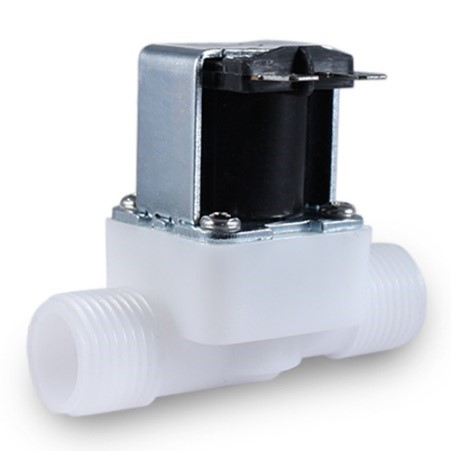
\includegraphics[width=3in]{8}
  \caption{12V DC solenoid valve [39].}\label{fig8}
\end{figure}

\subsection{DC Pump Specification}
\begin{enumerate}
  \item Dimension: 8 x 6 cm
  \item	Brushless pump power: 12V 960mA
  \item	Max water height: 6m
  \item	Max flow: 460LPH
  \item	Lifespan: not less than 20000 hours
  \item	Cable length: 40 cm
  \item	Color: black
  \item	The lead-out wire is 10 cm
  \item	Net weight: 200g
  \item	Package dimension: 88 x 56 x 70 mm
\end{enumerate}

Below Figure \ref{fig9} Shows a graphical illustration of 12 V DC Pump

\begin{figure}[h]
  \centering
  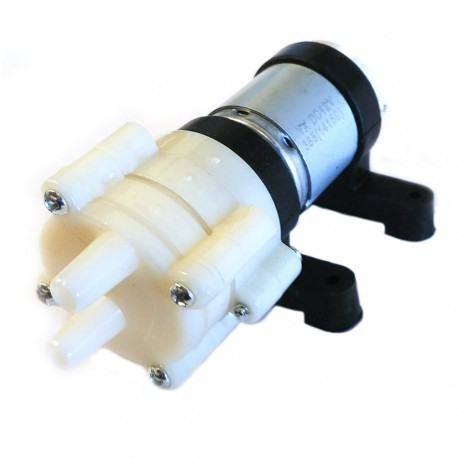
\includegraphics[width=3in]{9}
  \caption{DC Pump}\label{fig9}
\end{figure}

\section{Software Description}
Software tools that are used in the project

\begin{enumerate}
  \item	Arduino IDE (v1.0.6)
  \item	MySQL Database
\end{enumerate}

\subsection{Arduino IDE (v1.0.6)}
The Arduino integrated development environment (IDE) is a cross-platform application written in Java, and derives from the IDE for the Processing programming language and the Wiring projects. It is designed to introduce programming to artists and other newcomers unfamiliar with software development. It includes a code editor with features such as syntax highlighting, brace matching, and automatic indentation, and is also capable of compiling and uploading programs to the board with a single click. A program or code written for Arduino is called a "sketch". Figure \ref{fig10} shows the graphical picture of Arduino-IDE [40].


\begin{figure}[h]
  \centering
  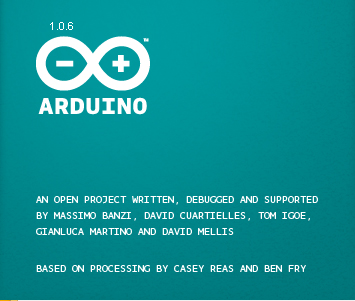
\includegraphics[width=4in]{10}
  \caption{Arduino-IDE lookout}\label{fig10}
\end{figure}

Arduino programs are written in C or C++. The Arduino IDE comes with a software library called "Wiring" from the original Wiring project, which makes many common input/output operations much easier. The users need only to define two functions to make an executable cyclic executive program:

\begin{itemize}
  \item setup(): a function run once at the start of a program that can initialize settings
  \item	loop(): a function called repeatedly until the board powers off
\end{itemize}

A typical first program for a microcontroller simply blinks an LED on and off. In the Arduino environment, the user might write a program like this:

\#define LED\textunderscore PIN 13\\
void setup()\{\\
    pinMode(LED\textunderscore PIN, OUTPUT);~~~~~// Enable pin 13 for digital output\\
\}\\
void loop()\{\\
    digitalWrite(LED\textunderscore PIN, HIGH);~~~~// Turn on the LED\\
    delay(1000);~~~~// Wait one second (1000 milliseconds)\\
    digitalWrite(LED\textunderscore PIN, LOW);~~~~~// Turn off the LED\\
    delay(1000);~~~~~// Wait one second\\
\}\\

It is a feature of most Arduino boards that they have an LED and load resistor connected between pin 13 and ground; a convenient feature for many simple tests. The previous code would not be seen by a standard C++ compiler as a valid program, so when the user clicks the "Upload to I/O board" button in the IDE, a copy of the code is written to a temporary file with an extra include header at the top and a very simple main() function at the bottom, to make it a valid C++ program. The Arduino IDE uses the GNU tool chain and AVR Libc to compile programs, and uses avrdude to upload programs to the board. As the Arduino platform uses Atmel microcontrollers, Atmel's development environment, AVR Studio or the newer Atmel Studio, may also be used to develop software for the Arduino \cite{cohen2018automated}.

\subsection{MySQL database}
MySQL is written in C and C++. Its SQL parser is written in yacc, but it uses a home brewed lexicalanalyzer. MySQLworksonmany systemplatforms,including AIX, BSDi, FreeBSD,HPUX, eComStation, i5/OS, IRIX, Linux, macOS, MicrosoftWindows, NetBSD, Novell,NetWare, OpenBSD, OpenSolaris, OS/2 Warp, QNX, Oracle Solaris, Symbian, SunOS, OpenServer, SCO UnixWare, Sanos and Tru64. A port of MySQL to OpenVMS also exists. The MySQL server software itself and the client libraries use dual-licensing distribution \cite{ercan2017rf}. They are offered under GPL version 2, or a proprietary license. Support can be obtained from the official manual. Free support additionally is available in different IRC channels and forums. Oracle offers paid support via its MySQL Enterprise products. They differ in the scope of services and in price. Additionally, a number of third party organizations exist to provide support and services, including MariaDB and Percona.

\begin{figure}
  \centering
  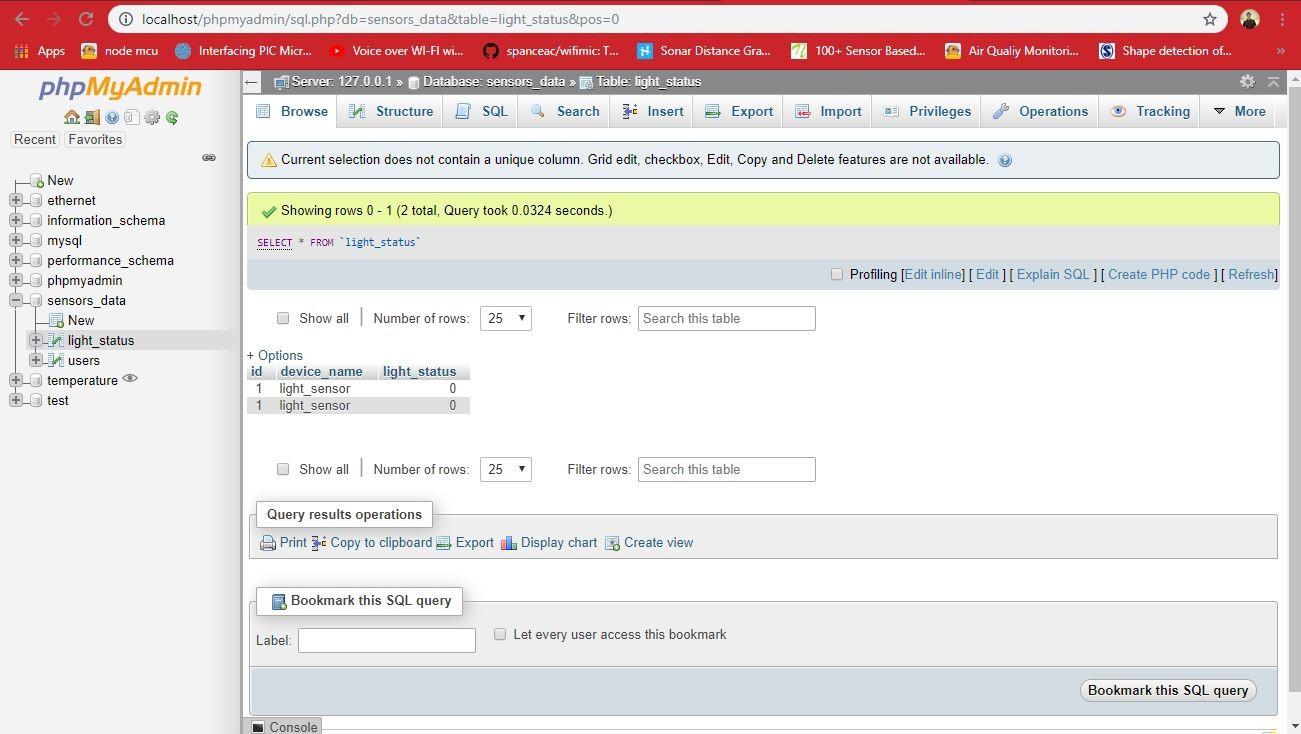
\includegraphics[width=4in,height=2.5 in]{11}
  \caption{Php My Admin console}\label{fig11}
\end{figure}
\section{Chapter Summery}
This chapter contained the details specification of the components used in this project implementation and their power rating.The components were divided into two sections.Every Section contains the proper details about their (components)uses and characteristics. 